% Informe de la práctica: control de un robot mediante gestos con una CNN.
% Compilar desde informe/:  latexmk -pdf -jobname=informe main.tex   (las cifras salen de generado/resultados.tex,
% que escribe src/analysis.py; las figuras se leen de ../results/)
\documentclass[11pt,a4paper]{article}

\usepackage[T1]{fontenc}
\usepackage[utf8]{inputenc}
\usepackage{lmodern}
\usepackage[spanish,es-tabla,es-nodecimaldot,es-noshorthands]{babel}
\spanishplainpercent        % \% normal (con babel-spanish falla dentro de $...$)
\usepackage[a4paper,margin=2.5cm]{geometry}
\usepackage{microtype}
\usepackage{amsmath,amssymb,bm}
\usepackage{graphicx}
\usepackage{booktabs}
\usepackage{float}
\usepackage[font=small,labelfont=bf]{caption}
\usepackage{subcaption}
\usepackage[inline]{enumitem}
\usepackage[dvipsnames]{xcolor}
\usepackage{tikz}
\usetikzlibrary{positioning,arrows.meta,shapes.geometric,fit,calc}
\usepackage[most]{tcolorbox}
\usepackage[numbers,sort&compress]{natbib}
\usepackage[hidelinks]{hyperref}
\usepackage[spanish,noabbrev]{cleveref}
\crefname{table}{tabla}{tablas}\Crefname{table}{Tabla}{Tablas}
\usepackage{fancyhdr}

\graphicspath{{../results/}}
\setlist{itemsep=2pt,topsep=4pt}
\setlength{\parskip}{3pt}

\pagestyle{fancy}
\fancyhf{}
\fancyhead[L]{\small Control de un robot mediante gestos con una CNN}
\fancyhead[R]{\small Aprendizaje Automático 2}
\fancyfoot[C]{\small\thepage}
\renewcommand{\headrulewidth}{0.4pt}

% Huecos que debe completar Carlos (sección de la demo)
\newtcolorbox{pendientebox}{colback=Apricot!15,colframe=BurntOrange,boxrule=0.6pt,arc=2pt,
  left=4pt,right=4pt,top=2pt,bottom=2pt,fontupper=\small}
\newcommand{\pendiente}[1]{\begin{pendientebox}\textbf{Pendiente (Carlos):} #1\end{pendientebox}}

\newcommand{\cls}[1]{\textit{#1}}          % nombre de clase de HaGRID
\newcommand{\code}[1]{\texttt{#1}}

% Generado por src/analysis.py a partir de results/: no editar a mano.

\newcommand{\NTrain}{11.088}
\newcommand{\PersonasTrain}{3.416}
\newcommand{\NVal}{2.375}
\newcommand{\PersonasVal}{735}
\newcommand{\NTest}{2.374}
\newcommand{\PersonasTest}{726}
\newcommand{\NTotal}{15.837}
\newcommand{\PersonasTotal}{4.877}
\newcommand{\PersonasCompartidas}{0}
\newcommand{\NImagenesOrig}{14.078}
\newcommand{\NManos}{17.296}
\newcommand{\NPersonasOrig}{4.877}
\newcommand{\NoGestureOrig}{3.219}
\newcommand{\NoGestureKept}{1.760}
\newcommand{\LadoCajaMediana}{68\,px}
\newcommand{\LadoCajaPdiez}{36\,px}
\newcommand{\AccValFinal}{98{,}99\,\%}
\newcommand{\FoneValFinal}{98{,}99\,\%}
\newcommand{\ErroresValFinal}{24}
\newcommand{\AccTestFinal}{98{,}99\,\%}
\newcommand{\FoneTestFinal}{98{,}99\,\%}
\newcommand{\ErroresTestFinal}{24}
\newcommand{\EpocasFinal}{44}
\newcommand{\MejorepocaFinal}{38}
\newcommand{\ReduccioneslrFinal}{22, 32 y 43}
\newcommand{\NreduccioneslrFinal}{3}
\newcommand{\AccepocaunoFinal}{25{,}7\,\%}
\newcommand{\EpocanoventaycincoFinal}{7}
\newcommand{\BrechaFinal}{0{,}5}
\newcommand{\AccValCompleto}{98{,}99\,\%}
\newcommand{\FoneValCompleto}{98{,}99\,\%}
\newcommand{\ErroresValCompleto}{24}
\newcommand{\AccTestCompleto}{98{,}99\,\%}
\newcommand{\FoneTestCompleto}{98{,}99\,\%}
\newcommand{\ErroresTestCompleto}{24}
\newcommand{\EpocasCompleto}{44}
\newcommand{\MejorepocaCompleto}{38}
\newcommand{\ReduccioneslrCompleto}{22, 32 y 43}
\newcommand{\NreduccioneslrCompleto}{3}
\newcommand{\AccepocaunoCompleto}{25{,}7\,\%}
\newcommand{\EpocanoventaycincoCompleto}{7}
\newcommand{\BrechaCompleto}{0{,}5}
\newcommand{\AccValCompletoS}{98{,}82\,\%}
\newcommand{\FoneValCompletoS}{98{,}82\,\%}
\newcommand{\ErroresValCompletoS}{28}
\newcommand{\AccTestCompletoS}{99{,}03\,\%}
\newcommand{\FoneTestCompletoS}{99{,}03\,\%}
\newcommand{\ErroresTestCompletoS}{23}
\newcommand{\EpocasCompletoS}{34}
\newcommand{\MejorepocaCompletoS}{28}
\newcommand{\ReduccioneslrCompletoS}{15 y 33}
\newcommand{\NreduccioneslrCompletoS}{2}
\newcommand{\AccepocaunoCompletoS}{25{,}3\,\%}
\newcommand{\EpocanoventaycincoCompletoS}{9}
\newcommand{\BrechaCompletoS}{0{,}3}
\newcommand{\AccValSinDropout}{98{,}95\,\%}
\newcommand{\FoneValSinDropout}{98{,}95\,\%}
\newcommand{\ErroresValSinDropout}{25}
\newcommand{\AccTestSinDropout}{98{,}82\,\%}
\newcommand{\FoneTestSinDropout}{98{,}82\,\%}
\newcommand{\ErroresTestSinDropout}{28}
\newcommand{\EpocasSinDropout}{29}
\newcommand{\MejorepocaSinDropout}{23}
\newcommand{\ReduccioneslrSinDropout}{13, 21 y 28}
\newcommand{\NreduccioneslrSinDropout}{3}
\newcommand{\AccepocaunoSinDropout}{51{,}2\,\%}
\newcommand{\EpocanoventaycincoSinDropout}{6}
\newcommand{\BrechaSinDropout}{1{,}1}
\newcommand{\AccValSinDropoutS}{99{,}12\,\%}
\newcommand{\FoneValSinDropoutS}{99{,}12\,\%}
\newcommand{\ErroresValSinDropoutS}{21}
\newcommand{\AccTestSinDropoutS}{99{,}12\,\%}
\newcommand{\FoneTestSinDropoutS}{99{,}11\,\%}
\newcommand{\ErroresTestSinDropoutS}{21}
\newcommand{\EpocasSinDropoutS}{50}
\newcommand{\MejorepocaSinDropoutS}{44}
\newcommand{\ReduccioneslrSinDropoutS}{22, 27, 35, 40 y 49}
\newcommand{\NreduccioneslrSinDropoutS}{5}
\newcommand{\AccepocaunoSinDropoutS}{56{,}2\,\%}
\newcommand{\EpocanoventaycincoSinDropoutS}{5}
\newcommand{\BrechaSinDropoutS}{0{,}9}
\newcommand{\AccValSinBn}{97{,}52\,\%}
\newcommand{\FoneValSinBn}{97{,}51\,\%}
\newcommand{\ErroresValSinBn}{59}
\newcommand{\AccTestSinBn}{97{,}68\,\%}
\newcommand{\FoneTestSinBn}{97{,}68\,\%}
\newcommand{\ErroresTestSinBn}{55}
\newcommand{\EpocasSinBn}{50}
\newcommand{\MejorepocaSinBn}{47}
\newcommand{\ReduccioneslrSinBn}{39}
\newcommand{\NreduccioneslrSinBn}{1}
\newcommand{\AccepocaunoSinBn}{16{,}8\,\%}
\newcommand{\EpocanoventaycincoSinBn}{25}
\newcommand{\BrechaSinBn}{-1{,}2}
\newcommand{\AccValSinBnS}{97{,}60\,\%}
\newcommand{\FoneValSinBnS}{97{,}60\,\%}
\newcommand{\ErroresValSinBnS}{57}
\newcommand{\AccTestSinBnS}{97{,}94\,\%}
\newcommand{\FoneTestSinBnS}{97{,}93\,\%}
\newcommand{\ErroresTestSinBnS}{49}
\newcommand{\EpocasSinBnS}{50}
\newcommand{\MejorepocaSinBnS}{49}
\newcommand{\ReduccioneslrSinBnS}{40}
\newcommand{\NreduccioneslrSinBnS}{1}
\newcommand{\AccepocaunoSinBnS}{14{,}6\,\%}
\newcommand{\EpocanoventaycincoSinBnS}{23}
\newcommand{\BrechaSinBnS}{-1{,}5}
\newcommand{\AccValSinAug}{98{,}65\,\%}
\newcommand{\FoneValSinAug}{98{,}65\,\%}
\newcommand{\ErroresValSinAug}{32}
\newcommand{\AccTestSinAug}{98{,}86\,\%}
\newcommand{\FoneTestSinAug}{98{,}86\,\%}
\newcommand{\ErroresTestSinAug}{27}
\newcommand{\EpocasSinAug}{23}
\newcommand{\MejorepocaSinAug}{17}
\newcommand{\ReduccioneslrSinAug}{15 y 22}
\newcommand{\NreduccioneslrSinAug}{2}
\newcommand{\AccepocaunoSinAug}{50{,}4\,\%}
\newcommand{\EpocanoventaycincoSinAug}{6}
\newcommand{\BrechaSinAug}{1{,}3}
\newcommand{\AccValSinAugS}{98{,}82\,\%}
\newcommand{\FoneValSinAugS}{98{,}82\,\%}
\newcommand{\ErroresValSinAugS}{28}
\newcommand{\AccTestSinAugS}{98{,}44\,\%}
\newcommand{\FoneTestSinAugS}{98{,}44\,\%}
\newcommand{\ErroresTestSinAugS}{37}
\newcommand{\EpocasSinAugS}{24}
\newcommand{\MejorepocaSinAugS}{18}
\newcommand{\ReduccioneslrSinAugS}{18 y 23}
\newcommand{\NreduccioneslrSinAugS}{2}
\newcommand{\AccepocaunoSinAugS}{50{,}5\,\%}
\newcommand{\EpocanoventaycincoSinAugS}{7}
\newcommand{\BrechaSinAugS}{1{,}3}
\newcommand{\AccValResnet}{99{,}41\,\%}
\newcommand{\FoneValResnet}{99{,}41\,\%}
\newcommand{\ErroresValResnet}{14}
\newcommand{\AccTestResnet}{99{,}20\,\%}
\newcommand{\FoneTestResnet}{99{,}20\,\%}
\newcommand{\ErroresTestResnet}{19}
\newcommand{\EpocasResnet}{23}
\newcommand{\MejorepocaResnet}{17}
\newcommand{\ReduccioneslrResnet}{10 y 22}
\newcommand{\NreduccioneslrResnet}{2}
\newcommand{\AccepocaunoResnet}{97{,}6\,\%}
\newcommand{\EpocanoventaycincoResnet}{1}
\newcommand{\BrechaResnet}{0{,}7}
\newcommand{\AccTestFinalIC}{[98{,}53\,\%;\ 99{,}40\,\%]}
\newcommand{\FoneTestFinalIC}{[98{,}53\,\%;\ 99{,}41\,\%]}
\newcommand{\NBoot}{2.000}
\newcommand{\AccTestResnetIC}{[98{,}76\,\%;\ 99{,}57\,\%]}
\newcommand{\FoneTestResnetIC}{[98{,}76\,\%;\ 99{,}58\,\%]}
\newcommand{\ConfusionesTestFinal}{\textit{like}$\to$\textit{call} (5), \textit{palm}$\to$\textit{stop} (4), \textit{stop}$\to$\textit{palm} (4), \textit{no\_gesture}$\to$\textit{like} (2)}
\newcommand{\PeorClaseTest}{\textit{palm}}
\newcommand{\PeorFoneTest}{98{,}1\,\%}
\newcommand{\FalsasActivaciones}{5}
\newcommand{\NNoGestureTest}{264}
\newcommand{\TasaFalsasActivaciones}{1{,}9\,\%}
\newcommand{\Omisiones}{1}
\newcommand{\ErroresEnPares}{13}
\newcommand{\AccValMediaCompleto}{98{,}91\,\%}
\newcommand{\AccTestMediaCompleto}{99{,}01\,\%}
\newcommand{\FoneValMediaCompleto}{98{,}91\,\%}
\newcommand{\FoneTestMediaCompleto}{99{,}01\,\%}
\newcommand{\AccValMediaSinDropout}{99{,}03\,\%}
\newcommand{\AccTestMediaSinDropout}{98{,}97\,\%}
\newcommand{\FoneValMediaSinDropout}{99{,}03\,\%}
\newcommand{\FoneTestMediaSinDropout}{98{,}97\,\%}
\newcommand{\AccValMediaSinBn}{97{,}56\,\%}
\newcommand{\AccTestMediaSinBn}{97{,}81\,\%}
\newcommand{\FoneValMediaSinBn}{97{,}55\,\%}
\newcommand{\FoneTestMediaSinBn}{97{,}80\,\%}
\newcommand{\AccValMediaSinAug}{98{,}74\,\%}
\newcommand{\AccTestMediaSinAug}{98{,}65\,\%}
\newcommand{\FoneValMediaSinAug}{98{,}74\,\%}
\newcommand{\FoneTestMediaSinAug}{98{,}65\,\%}
\newcommand{\PmcnemarSinDropout}{$p = 0{,}541$}
\newcommand{\SolocompletoSinDropout}{14}
\newcommand{\SolovarianteSinDropout}{10}
\newcommand{\PmcnemarSinBn}{$p < 0{,}001$}
\newcommand{\SolocompletoSinBn}{42}
\newcommand{\SolovarianteSinBn}{11}
\newcommand{\PmcnemarSinAug}{$p = 0{,}701$}
\newcommand{\SolocompletoSinAug}{15}
\newcommand{\SolovarianteSinAug}{12}
\newcommand{\PmcnemarResnet}{$p = 0{,}424$}
\newcommand{\SolocompletoResnet}{10}
\newcommand{\SolovarianteResnet}{15}
\newcommand{\VersionTorch}{2.14.1}
\newcommand{\GPU}{GTX 1660 Ti}
\newcommand{\CPU}{Intel Core i7-9750H @ 2.60GHz}
\newcommand{\CPUHilos}{6}
\newcommand{\ParamsFinal}{2{,}36\,M}
\newcommand{\MacsFinal}{920\,M}
\newcommand{\LatCpuFinal}{8{,}68\,ms}
\newcommand{\LatCudaFinal}{1{,}03\,ms}
\newcommand{\SepocaFinal}{25{,}5\,s}
\newcommand{\ParamsResnet}{11{,}18\,M}
\newcommand{\MacsResnet}{592\,M}
\newcommand{\LatCpuResnet}{10{,}23\,ms}
\newcommand{\LatCudaResnet}{2{,}07\,ms}
\newcommand{\SepocaResnet}{12{,}1\,s}
\newcommand{\FracMacsPrimerosBloques}{43\,\%}
\newcommand{\FracParamsPrimerosBloques}{3\,\%}
\newcommand{\RatioParams}{4{,}7}
\newcommand{\RatioMacs}{1{,}6}
\newcommand{\RatioSEpoca}{2{,}1}

\newcommand{\TablaDatos}{%
\begin{tabular}{llrrrr}
\toprule
Clase & Orden & Train & Val & Test & Total \\
\midrule
\textit{stop} & Parar & 1225 & 261 & 262 & 1748 \\
\textit{like} & Avanzar & 1214 & 258 & 260 & 1732 \\
\textit{dislike} & Retroceder & 1248 & 268 & 267 & 1783 \\
\textit{one} & Girar a la izquierda & 1245 & 267 & 266 & 1778 \\
\textit{peace} & Girar a la derecha & 1237 & 266 & 266 & 1769 \\
\textit{fist} & Cerrar pinza & 1214 & 259 & 261 & 1734 \\
\textit{palm} & Abrir pinza & 1239 & 267 & 264 & 1770 \\
\textit{call} & Volver al inicio & 1234 & 265 & 264 & 1763 \\
\textit{no\_gesture} & Ninguna (quieto) & 1232 & 264 & 264 & 1760 \\
\midrule
Total imágenes & & 11088 & 2375 & 2374 & 15837 \\
Personas & & 3416 & 735 & 726 & 4877 \\
\bottomrule
\end{tabular}}

\newcommand{\TablaAblacion}{%
\begin{tabular}{lccc cc cc c}
\toprule
& & & & \multicolumn{2}{c}{Validación} & \multicolumn{2}{c}{Test} & \\
\cmidrule(lr){5-6}\cmidrule(lr){7-8}
Variante & Dropout & BN & Augm. & Acc. & F1 macro & Acc. & F1 macro & Épocas \\
\midrule
Completo & sí & sí & sí & 98{,}91\,\% & 98{,}91\,\% & 99{,}01\,\% & 99{,}01\,\% & 44 / 34 \\
Sin dropout & no & sí & sí & 99{,}03\,\% & 99{,}03\,\% & 98{,}97\,\% & 98{,}97\,\% & 29 / 50 \\
Sin BN & sí & no & sí & 97{,}56\,\% & 97{,}55\,\% & 97{,}81\,\% & 97{,}80\,\% & 50 / 50 \\
Sin augmentation & sí & sí & no & 98{,}74\,\% & 98{,}74\,\% & 98{,}65\,\% & 98{,}65\,\% & 23 / 24 \\
\midrule
ResNet18 preentrenado$^\dagger$ & — & sí & sí & 99{,}41\,\% & 99{,}41\,\% & 99{,}20\,\% & 99{,}20\,\% & 23 \\
\bottomrule
\end{tabular}}

\newcommand{\TablaSemillas}{%
\begin{tabular}{l rr rr rrr}
\toprule
& \multicolumn{2}{c}{Acc. val} & \multicolumn{2}{c}{Errores test} & \multicolumn{3}{c}{McNemar vs.\ completo (semilla 42)} \\
\cmidrule(lr){2-3}\cmidrule(lr){4-5}\cmidrule(lr){6-8}
Variante & s42 & s43 & s42 & s43 & solo compl. & solo var. & $p$ \\
\midrule
Completo & 98{,}99\,\% & 98{,}82\,\% & 24 & 23 & — & — & — \\
Sin dropout & 98{,}95\,\% & 99{,}12\,\% & 28 & 21 & 14 & 10 & 0{,}541 \\
Sin BN & 97{,}52\,\% & 97{,}60\,\% & 55 & 49 & 42 & 11 & $<\!0{,}001$ \\
Sin augmentation & 98{,}65\,\% & 98{,}82\,\% & 27 & 37 & 15 & 12 & 0{,}701 \\
\midrule
ResNet18 preentrenado & 99{,}41\,\% & — & 19 & — & 10 & 15 & 0{,}424 \\
\bottomrule
\end{tabular}}

\newcommand{\TablaPorClase}{%
\begin{tabular}{llrrrr}
\toprule
Clase & Orden & Precisión & Recall & F1 & $n$ \\
\midrule
\textit{stop} & Parar & 98{,}5\,\% & 98{,}5\,\% & 98{,}5\,\% & 262 \\
\textit{like} & Avanzar & 99{,}2\,\% & 97{,}3\,\% & 98{,}3\,\% & 260 \\
\textit{dislike} & Retroceder & 100{,}0\,\% & 100{,}0\,\% & 100{,}0\,\% & 267 \\
\textit{one} & Girar a la izquierda & 99{,}3\,\% & 99{,}6\,\% & 99{,}4\,\% & 266 \\
\textit{peace} & Girar a la derecha & 98{,}9\,\% & 99{,}2\,\% & 99{,}1\,\% & 266 \\
\textit{fist} & Cerrar pinza & 100{,}0\,\% & 99{,}6\,\% & 99{,}8\,\% & 261 \\
\textit{palm} & Abrir pinza & 97{,}7\,\% & 98{,}5\,\% & 98{,}1\,\% & 264 \\
\textit{call} & Volver al inicio & 97{,}8\,\% & 100{,}0\,\% & 98{,}9\,\% & 264 \\
\textit{no\_gesture} & Ninguna (quieto) & 99{,}6\,\% & 98{,}1\,\% & 98{,}9\,\% & 264 \\
\bottomrule
\end{tabular}}

\newcommand{\TablaCoste}{%
\begin{tabular}{lrrrrrrr}
\toprule
& & & & \multicolumn{2}{c}{CPU (ms)} & \multicolumn{2}{c}{GPU (ms)} \\
\cmidrule(lr){5-6}\cmidrule(lr){7-8}
Modelo & Parámetros & MACs & s/época & mediana & p95 & mediana & p95 \\
\midrule
GestureCNN & 2{,}36\,M & 920\,M & 25{,}5 & 8{,}68 & 9{,}62 & 1{,}03 & 1{,}07 \\
ResNet18 & 11{,}18\,M & 592\,M & 12{,}1 & 10{,}23 & 10{,}62 & 2{,}07 & 2{,}29 \\
\bottomrule
\end{tabular}}



\title{\textbf{Control de un robot mediante gestos de la mano\\con una red convolucional entrenada desde cero}}
\author{Daniel Rodríguez Alonso \and Carlos Falcón Brito}
\date{Aprendizaje Automático 2 · Práctica de redes convolucionales\\[2pt] 31 de octubre de 2026}

\begin{document}
\maketitle
\thispagestyle{empty}

\begin{abstract}
\noindent
Este trabajo estudia si una red convolucional pequeña, entrenada desde cero, puede reconocer con
fiabilidad un vocabulario de gestos de la mano pensado para dar órdenes a un robot.
Partimos de un subconjunto de HaGRID con ocho gestos (\cls{stop}, \cls{like}, \cls{dislike},
\cls{one}, \cls{peace}, \cls{fist}, \cls{palm} y \cls{call}) y una clase nula
(\cls{no\_gesture}) que deja el robot quieto. Clasificamos recortes de la mano de
$128\times128$\,px y dividimos los datos \emph{por persona}, de modo que las \PersonasTest{}
personas de test no aparecen en entrenamiento ni en validación.
La red propuesta, GestureCNN, tiene cinco bloques convolucionales con normalización por lotes,
\emph{dropout} y \emph{global average pooling} (\ParamsFinal{} parámetros). Tras una búsqueda
manual de \NConfigsBusqueda{} configuraciones, el modelo final se entrena con lotes de 32. En
test alcanza una
exactitud del \AccTestFinal{} (IC del 95\,\% por \emph{bootstrap} por persona: \AccTestFinalIC)
y una F1 macro del \FoneTestFinal, muy por encima del objetivo del 85\,\%.
Un estudio de ablación con dos semillas indica que la normalización por lotes es el componente
decisivo, mientras que el \emph{dropout} y el aumento de datos tienen efectos pequeños sobre la
exactitud con este conjunto de datos; la búsqueda de hiperparámetros muestra también una
sensibilidad baja a la tasa de aprendizaje, al lote, a la capacidad y a la activación. Un ResNet18 preentrenado en ImageNet sirve de referencia
(\AccTestResnet{} en test) con \RatioParams{} veces más parámetros. Los mapas Grad-CAM muestran que la red
atiende a los dedos que distinguen cada gesto, y los errores restantes se concentran en pares
visualmente próximos (\cls{stop}/\cls{palm}, \cls{like}/\cls{call}) y en ejemplos con ruido de
etiqueta. Por último, se describe el diseño de una demo en tiempo real con ROS\,2 y
\emph{turtlesim}.

\medskip\noindent\textbf{Palabras clave:} reconocimiento de gestos, redes convolucionales,
interacción persona-robot, HaGRID, ablación, Grad-CAM.
\end{abstract}

\section{Introducción}
\label{sec:introduccion}

Los gestos de la mano son una forma natural de dar órdenes a una máquina sin mando ni contacto.
Esta ventaja es especialmente útil en entornos ruidosos o industriales, donde la voz no es
fiable, o cuando el operador tiene las manos ocupadas y no puede manejar un mando
\citep{pisharady2015review}. Para un robot, sin embargo, no basta con reconocer gestos: hace falta
un \emph{vocabulario de órdenes} con un significado preciso para cada uno y, sobre todo, una forma
segura de no hacer nada. Por eso este trabajo plantea el problema como la clasificación de un
conjunto cerrado de órdenes más una \emph{clase nula} (\cls{no\_gesture}) que deja el robot
quieto, en lugar de como un reconocimiento de gestos arbitrarios.

Este planteamiento impone tres requisitos que guían todo el diseño experimental:
\begin{enumerate}
  \item \textbf{Robustez ante personas nuevas.} El robot tendrá que obedecer a personas que el
    modelo nunca vio. Por tanto, la estimación del rendimiento debe hacerse con personas ausentes
    del entrenamiento; una partición aleatoria por imagen sería optimista, porque la misma persona,
    con el mismo fondo y la misma iluminación, aparecería a ambos lados \citep{kaufman2012leakage}.
  \item \textbf{Una clase nula fiable.} Confundir una mano en reposo con una orden mueve el robot
    sin querer, que es el error más costoso en la práctica.
  \item \textbf{Bajo coste de inferencia.} La clasificación debe ejecutarse en tiempo real en un
    ordenador portátil, lo que favorece modelos pequeños.
\end{enumerate}

\paragraph{Objetivos.}
El objetivo principal es alcanzar al menos un 85\,\% de exactitud en test con personas no vistas,
usando una red convolucional diseñada y entrenada desde cero en PyTorch \citep{paszke2019pytorch}.
La red debe incluir convolución, \emph{pooling}, normalización por lotes y \emph{dropout}, y su
entrenamiento debe usar parada anticipada sobre la pérdida de validación con restauración de los
mejores pesos. Además, nos propusimos analizar el modelo con una matriz de confusión, mapas
Grad-CAM y un estudio de ablación (con y sin \emph{dropout}, normalización por lotes y aumento
de datos). Como extensiones opcionales, el plan incluía comparar con un ResNet18 preentrenado y
construir una demo en tiempo real que controle un robot simulado en ROS\,2.

\paragraph{Contribuciones.}
\begin{itemize}
  \item Un \emph{pipeline} de datos reproducible sobre HaGRID: recorte de manos a partir de las
    cajas anotadas, una clase nula construida con las manos que no hacen el gesto y una partición
    estratificada \emph{por persona} sin personas compartidas entre particiones
    (\cref{sec:datos}).
  \item GestureCNN, una red de \ParamsFinal{} parámetros que alcanza un \AccTestFinal{} de
    exactitud en test, con un intervalo de confianza que tiene en cuenta la dependencia entre
    imágenes de una misma persona (\cref{sec:resultados}).
  \item Un estudio de ablación con dos semillas y pruebas de McNemar pareadas, que separa los
    efectos reales de la variación entre ejecuciones (\cref{sec:ablacion}).
  \item Una comparación con ResNet18 que incluye el coste computacional (parámetros, operaciones y
    latencia) y un análisis cualitativo de los errores con Grad-CAM.
\end{itemize}

El resto del documento se organiza así: la \cref{sec:relacionado} resume el trabajo relacionado;
la \cref{sec:datos} describe los datos y la partición; la \cref{sec:metodos}, el preprocesado, la
arquitectura y el protocolo experimental; la \cref{sec:resultados} presenta los resultados; la
\cref{sec:demo}, el diseño de la demo; la \cref{sec:discusion} discute los resultados y sus
limitaciones, y la \cref{sec:conclusiones} concluye.

\section{Trabajo relacionado}
\label{sec:relacionado}

\paragraph{Conjuntos de datos de gestos.}
HaGRID \citep{kapitanov2024hagrid} es uno de los mayores conjuntos de imágenes de gestos de la
mano: su primera versión contiene 552\,992 imágenes FullHD de 18 gestos pensados para controlar
dispositivos, tomadas por miles de personas en entornos domésticos y con condiciones de
iluminación muy variadas. Cada imagen incluye las cajas de las manos, la etiqueta de cada mano
(las manos que no hacen el gesto se etiquetan como \cls{no\_gesture}) y un identificador
anónimo de la persona (\code{user\_id}), lo que permite particionar por persona. Usamos un
subconjunto público de 30\,000 imágenes reescaladas a 384\,px \citep{mills_hagridsample}.

\paragraph{Detector seguido de clasificador.}
En una imagen completa la mano ocupa muy pocos píxeles, así que los sistemas prácticos suelen
dividir el problema en dos etapas: un detector o rastreador de manos, como MediaPipe Hands
\citep{zhang2020mediapipe}, localiza la mano, y un clasificador decide el gesto a partir del
recorte \citep{pisharady2015review}. Este trabajo se centra en la segunda etapa: durante el
entrenamiento y la evaluación usamos las cajas anotadas, y el detector solo interviene en la
demo (\cref{sec:demo}).

\paragraph{Arquitecturas convolucionales.}
Nuestra red sigue el esquema de bloques de VGG \citep{simonyan2015vgg}: dos convoluciones
$3\times3$ seguidas de \emph{max pooling}. Le añade normalización por lotes (BN)
\citep{ioffe2015bn}, que estabiliza la distribución de las activaciones y permite tasas de
aprendizaje mayores, y \emph{dropout} \citep{srivastava2014dropout}, en su variante espacial
(\code{Dropout2d}) en los bloques convolucionales \citep{tompson2015spatialdropout}. En lugar de
capas densas grandes al final usa \emph{global average pooling} \citep{lin2014nin}, que reduce
mucho el número de parámetros. Como referencia de un modelo más grande usamos ResNet18
\citep{he2016resnet} preentrenado en ImageNet \citep{deng2009imagenet}; ajustar una red
preentrenada aprovecha rasgos genéricos de las primeras capas que se transfieren bien a otras
tareas \citep{yosinski2014transferable}.

\paragraph{Explicabilidad y evaluación.}
Grad-CAM \citep{selvaraju2017gradcam} genera mapas de calor que indican qué regiones de la
imagen empujan la predicción hacia una clase, a partir de los gradientes en la última capa
convolucional. Lo usamos para comprobar que la red mira la mano y no el fondo. Para comparar
clasificadores evaluados sobre el mismo conjunto de test usamos la prueba de McNemar
\citep{mcnemar1947}, recomendada para este escenario por \citet{dietterich1998tests}, e
intervalos de confianza por \emph{bootstrap} \citep{efron1993bootstrap}.

\section{Datos}
\label{sec:datos}

Usamos el subconjunto público \code{hagrid-sample-30k-384p} \citep{mills_hagridsample} de HaGRID,
con imágenes de 384\,px y las anotaciones originales: la caja de cada mano, su etiqueta y un
identificador anónimo de la persona (\code{user\_id}). Elegimos los ocho gestos de la
\cref{tab:datos}, que cubren las órdenes básicas de un robot móvil con pinza. Sus
\NImagenesOrig{} imágenes contienen \NManos{} manos de \NPersonasOrig{} personas. La clase nula
está formada por las \NoGestureOrig{} \emph{segundas manos} de esas mismas imágenes, que HaGRID
etiqueta como \cls{no\_gesture} porque no hacen el gesto. Así, los negativos comparten persona,
fondo e iluminación con los positivos, y la red no puede separar las clases por el contexto. Para
equilibrar las clases, submuestreamos la nula hasta \NoGestureKept{} ejemplos, el tamaño medio de
una clase de gesto.

Cada mano se recorta como un cuadrado centrado en su caja, de lado 1,5 veces el lado mayor de la
caja (un margen del 25\,\% por cada lado), y se redimensiona a $128\times128$\,px
(\cref{fig:recortes}). Las manos son pequeñas (la mediana del lado de la caja es de
\LadoCajaMediana), así que la mayoría de los recortes se amplían.

La partición usa \code{StratifiedGroupKFold} con \code{user\_id} como grupo: 20 trozos
estratificados por clase, de los que 14 van a entrenamiento, 3 a validación y 3 a test
(70/15/15). Resultan \NTrain{}, \NVal{} y \NTest{} recortes de \PersonasTrain{}, \PersonasVal{} y
\PersonasTest{} personas, sin ninguna persona compartida entre particiones (lo comprueba una
prueba automática). La normalización por canal usa estadísticas calculadas solo con
entrenamiento.

\begin{table}[t]
  \centering
  \caption{Vocabulario de órdenes y recortes por clase y partición, tras equilibrar
    \cls{no\_gesture}. Ninguna persona aparece en más de una partición.}
  \label{tab:datos}
  \small
  \TablaDatos
\end{table}

\begin{figure}[t]
  \centering
  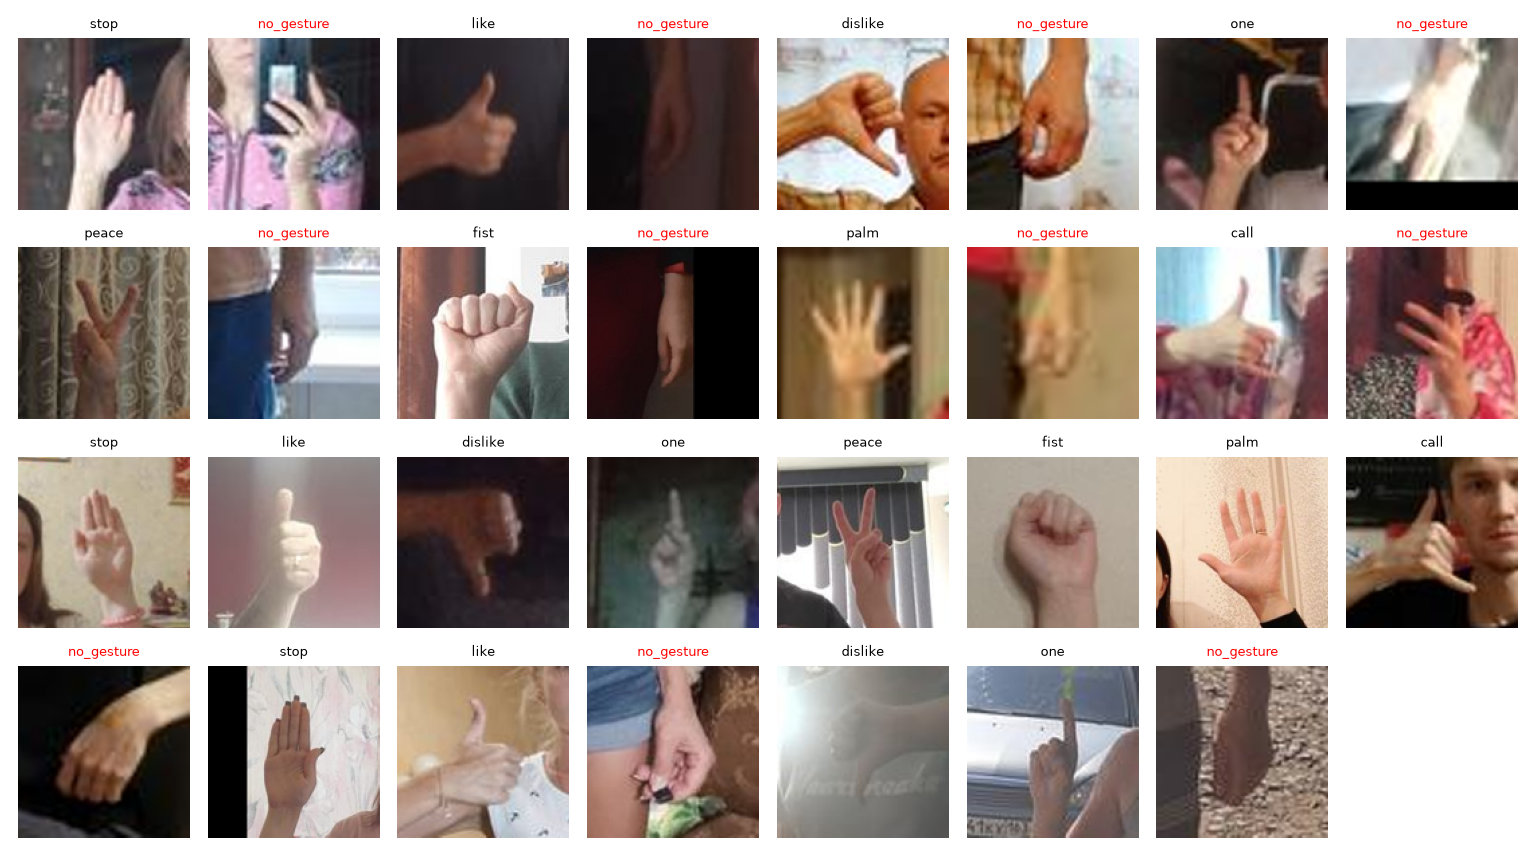
\includegraphics[width=0.8\linewidth]{figures/recortes_muestra.png}
  \caption{Recortes de $128\times128$\,px de las nueve clases. Los de \cls{no\_gesture} (en rojo)
    son manos en reposo, sujetando objetos o parcialmente visibles.}
  \label{fig:recortes}
\end{figure}

\section{Métodos}
\label{sec:metodos}

\paragraph{Aumento de datos.}
En entrenamiento, cada recorte se rota hasta $\pm15^\circ$, se recorta al azar conservando entre
el 80 y el 100\,\% del área (\code{RandomResizedCrop} con aspecto 1:1), se voltea horizontalmente
con probabilidad 0,5 y se varían el brillo y el contraste ($\pm30\,\%$) y la saturación
($\pm20\,\%$) \citep{shorten2019augmentation}. Ninguna de estas transformaciones cambia el
significado del gesto. Por eso se excluye el volteo vertical, que convierte \cls{like} en
\cls{dislike}.

\paragraph{Arquitectura.}
GestureCNN (\cref{fig:arquitectura}) encadena cinco bloques. Cada uno aplica dos veces la
secuencia convolución $3\times3$, BN y ReLU, y termina con un \emph{max pooling} $2\times2$. Los
canales crecen de 32 a 256 mientras la resolución baja de $128^2$ a $4^2$. Los tres últimos
bloques añaden \code{Dropout2d} (0,1, 0,2 y 0,3), que apaga mapas de características completos
\citep{tompson2015spatialdropout}. La cabeza aplica \emph{global average pooling}, un
\emph{dropout} de 0,5 y una capa lineal de 256 a 9 salidas: 2\,313 parámetros, frente a los
36\,873 de una capa lineal sobre el mapa aplanado. Las variantes de la ablación quitan BN o el
\emph{dropout} y dejan intacto el resto de la red.

\begin{figure}[t]
  \centering
  \begin{tikzpicture}[
      font=\footnotesize,
      blk/.style={draw, rounded corners=2pt, minimum height=1.25cm, minimum width=1.45cm,
                  align=center, fill=#1},
      arr/.style={-{Stealth[length=2mm]}, thick}]
    \node[blk=gray!10]   (in) {Entrada\\$3\times128^2$};
    \node[blk=blue!10,   right=0.35cm of in]  (b1) {Bloque 1\\32 c.\\$\to 64^2$};
    \node[blk=blue!10,   right=0.35cm of b1]  (b2) {Bloque 2\\64 c.\\$\to 32^2$};
    \node[blk=blue!18,   right=0.35cm of b2]  (b3) {Bloque 3\\128 c.\\$\to 16^2$\\{\scriptsize drop 0,1}};
    \node[blk=blue!26,   right=0.35cm of b3]  (b4) {Bloque 4\\256 c.\\$\to 8^2$\\{\scriptsize drop 0,2}};
    \node[blk=blue!34,   right=0.35cm of b4]  (b5) {Bloque 5\\256 c.\\$\to 4^2$\\{\scriptsize drop 0,3}};
    \node[blk=orange!15, right=0.35cm of b5]  (gap) {GAP\\256};
    \node[blk=orange!15, right=0.35cm of gap] (fc) {Dropout 0,5\\Lineal\\$256\to9$};
    \foreach \a/\b in {in/b1,b1/b2,b2/b3,b3/b4,b4/b5,b5/gap,gap/fc} \draw[arr] (\a) -- (\b);
    \node[below=0.45cm of b3, draw, dashed, rounded corners=2pt, align=left, inner sep=4pt,
          font=\scriptsize] (det)
      {Cada bloque: $[\text{Conv }3{\times}3 \to \text{BN} \to \text{ReLU}]\times2 \to
       \text{MaxPool }2{\times}2\ (\to \text{Dropout2d})$};
    \draw[dashed, gray] (det.north) -- (b3.south);
    \node[above=0.12cm of b5, font=\scriptsize, text=red!70!black, align=center]
      {Grad-CAM: 2.ª conv. ($256\times8^2$)};
  \end{tikzpicture}
  \caption{Arquitectura de GestureCNN (\ParamsFinal{} parámetros): canales, resolución de salida
    y probabilidad de \code{Dropout2d} de cada bloque. Grad-CAM se calcula sobre la última
    convolución.}
  \label{fig:arquitectura}
\end{figure}

\paragraph{Entrenamiento.}
Usamos entropía cruzada sin pesos de clase, porque las clases están equilibradas, y Adam
\citep{kingma2015adam} con una tasa de aprendizaje inicial de $10^{-3}$, \emph{weight decay}
$10^{-4}$ y lotes de 64 (32 en el modelo final). La tasa se divide por dos tras 3 épocas sin mejorar
la pérdida de validación. La parada anticipada \citep{prechelt1998early} detiene el entrenamiento
tras 6 épocas sin mejora, con un máximo de 50, y restaura los pesos de la mejor época. La semilla
es 42 salvo que se indique otra. Todo se entrenó con PyTorch \VersionTorch{} en una \GPU{} de
portátil. Como referencia, ResNet18 preentrenado en ImageNet \citep{deng2009imagenet} se reajusta
entero con el mismo protocolo, una capa final de 9 salidas y una tasa diez veces menor
($10^{-4}$).

\subsection{Búsqueda de hiperparámetros}
\label{sec:busqueda-metodo}

Partiendo del modelo completo (tasa $10^{-3}$, lotes de 64, cinco bloques de 32 a 256 filtros,
sin capa oculta y ReLU), hicimos una búsqueda manual en la que cada configuración cambia
\emph{un único} hiperparámetro y mantiene fijo todo lo demás, incluidas la semilla y la partición.
Probamos \NConfigsBusqueda{} configuraciones:
\begin{itemize}
  \item tasa de aprendizaje de $3\cdot10^{-4}$ y de $3\cdot10^{-3}$;
  \item lotes de 32 y de 128;
  \item la mitad de filtros por bloque (\ParamsFiltrosMitad{} parámetros), cuatro bloques en lugar
    de cinco (\ParamsCuatroBloques) y una capa oculta de 128 neuronas en la cabeza;
  \item activaciones ELU \citep{clevert2016elu} y LeakyReLU (pendiente 0,1) en lugar de ReLU.
\end{itemize}
Cada configuración se entrenó una vez y se evaluó solo en validación. El criterio de elección,
fijado de antemano, fue la exactitud de validación. Cambiar un único factor cada vez permite
atribuirle la diferencia y cuesta una ejecución por valor probado, unos 20 minutos; a cambio, no
explora interacciones entre hiperparámetros.

\subsection{Protocolo de evaluación}
\label{sec:protocolo}

\paragraph{Selección del modelo.}
Todas las decisiones se tomaron con validación, pero el modelo final se eligió en dos fases. Lo
indicamos explícitamente porque afecta a la lectura del test. Primero, el modelo final fue la
variante completa, que era la mejor en validación de la ablación. Con ella, con las variantes y
con ResNet18 se evaluó el test una vez por modelo. Después hicimos la búsqueda de
hiperparámetros, solo con validación. La configuración con lotes de 32 fue la mejor y pasó a ser el
modelo final. La decisión se tomó antes de evaluar esa configuración en test, donde también se
evaluó una sola vez; pero el test ya se había mirado con el modelo anterior. Por eso presentamos
y comparamos los dos (\cref{sec:test}).

\paragraph{Métricas e incertidumbre.}
Reportamos la exactitud, la F1 macro y la matriz de confusión normalizada por filas, cuya
diagonal es el \emph{recall}. Como las imágenes de una misma persona no son independientes, los
intervalos de confianza del 95\,\% se calculan por \emph{bootstrap} remuestreando \emph{personas}
(\NBoot{} réplicas) \citep{efron1993bootstrap}. Para comparar dos modelos sobre las mismas
imágenes de test usamos la prueba exacta de McNemar \citep{mcnemar1947,dietterich1998tests}, y
repetimos la ablación con una segunda semilla (43) para medir la variación entre ejecuciones.
Estas comparaciones son exploratorias y no se corrigen por comparaciones múltiples. Grad-CAM
\citep{selvaraju2017gradcam} se calcula sobre la última convolución ($8\times8$) y siempre en
validación.

\section{Resultados}
\label{sec:resultados}

\subsection{Búsqueda de hiperparámetros}
\label{sec:busqueda}

\begin{table}[t]
  \centering
  \caption{Búsqueda manual de hiperparámetros, solo en validación (\NVal{} imágenes). Cada fila
    cambia un único hiperparámetro de la referencia (tasa $10^{-3}$, lote de 64, cinco bloques de
    32 a 256 filtros, sin capa oculta, ReLU); todas usan la semilla 42. Pérdida: pérdida de
    validación en la mejor época. En negrita, la configuración elegida como modelo final.}
  \label{tab:busqueda}
  \small
  \setlength{\tabcolsep}{3.3pt}
  \TablaBusqueda
\end{table}

\begin{figure}[t]
  \centering
  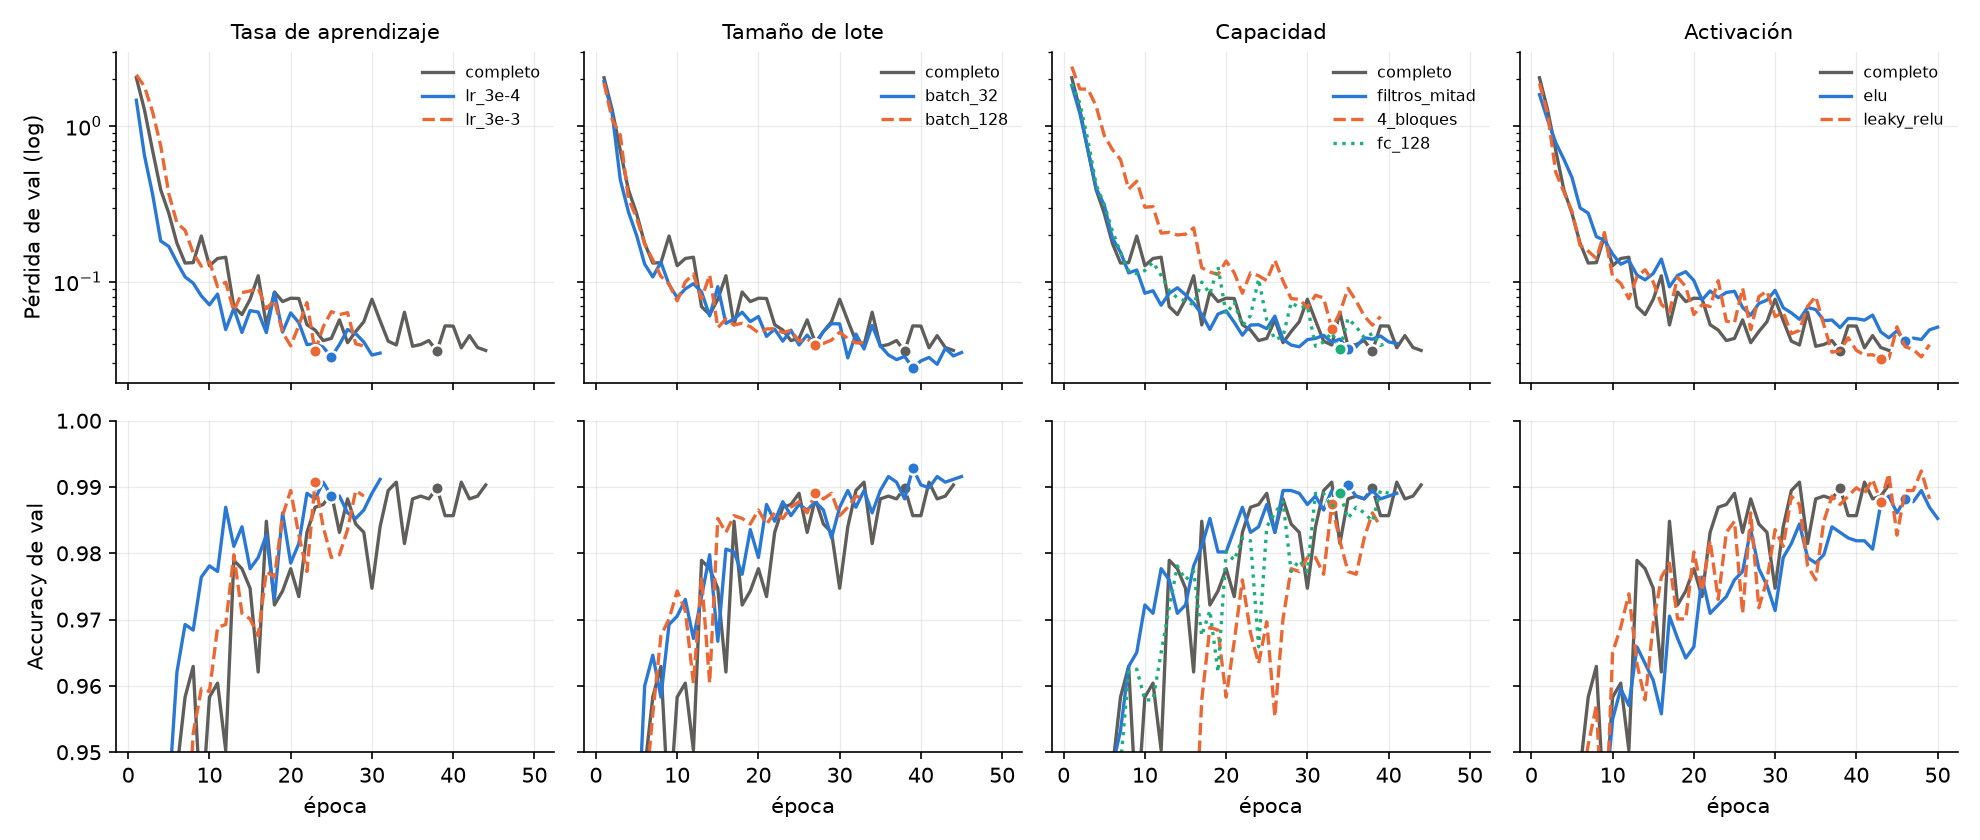
\includegraphics[width=\linewidth]{figures/busqueda_curvas.png}
  \caption{Curvas de validación de la búsqueda, un panel por tipo de hiperparámetro; en gris, la
    referencia. Arriba, la pérdida (escala logarítmica); abajo, la exactitud por encima del
    95\,\%. El punto marca la mejor época.}
  \label{fig:busqueda}
\end{figure}

La red es poco sensible a los cambios probados (\cref{tab:busqueda,fig:busqueda}): salvo el lote
de 32, todas las configuraciones quedan entre el \AccValBusquedaMin{} y el \AccValBusquedaMax{} de
exactitud de validación, a pocas imágenes de la referencia (\AccValCompleto). Para dar una medida
del ruido, dos ejecuciones idénticas del modelo completo con distinta semilla obtienen
\AccValCompleto{} y \AccValCompletoS. Con las tasas de $3\cdot10^{-3}$ y $3\cdot10^{-4}$ la parada
anticipada actúa antes (épocas \EpocasLrAlta{} y 31, frente a \EpocasCompleto), sin cambiar la
exactitud. Con la mitad de filtros la red rinde igual (\AccValFiltrosMitad) con cuatro veces menos
parámetros, lo que indica que está sobredimensionada. Quitar el último bloque es el cambio que más
empeora el resultado y el que más ralentiza el aprendizaje. La capa oculta no aporta nada, y ELU y
LeakyReLU quedan algo por debajo de ReLU.

El único cambio que mejora a la vez la exactitud y la pérdida de validación es el lote de 32
(\ErroresValFinal{} errores, frente a \ErroresValCompleto): con la misma tasa, da el doble de
actualizaciones por época y un gradiente más ruidoso, que actúa como regularizador. Según el
criterio fijado, pasa a ser el modelo final. Aun así, su ventaja procede de una sola ejecución y de
elegir la mejor de diez configuraciones, así que su exactitud de validación tiende a ser optimista.

\subsection{Modelo final}
\label{sec:test}

\begin{figure}[t]
  \centering
  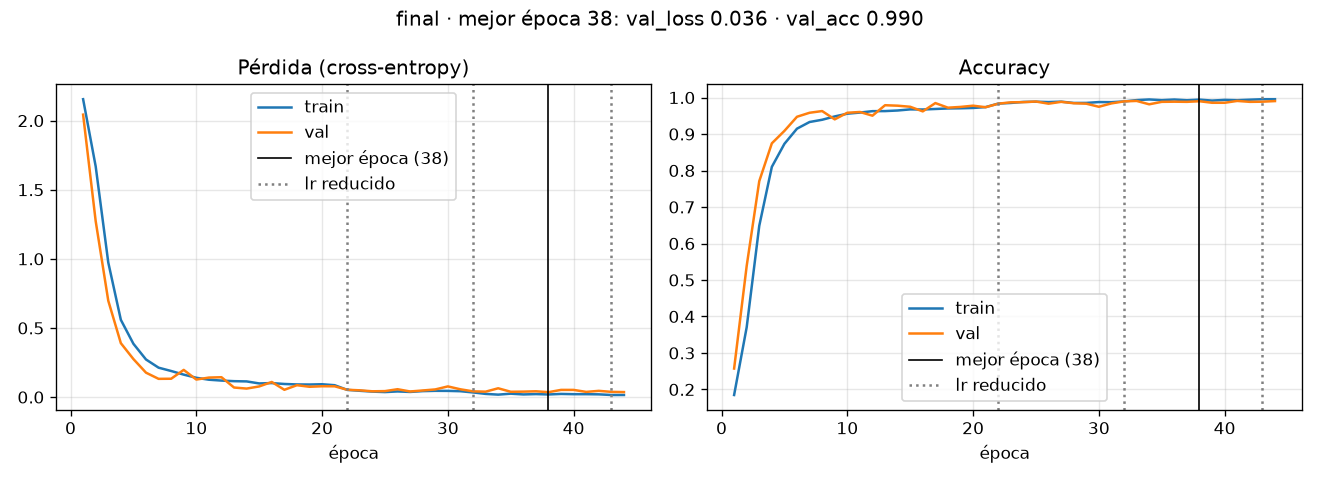
\includegraphics[width=0.92\linewidth]{final/curves.png}
  \caption{Pérdida y exactitud de entrenamiento y validación del modelo final (lotes de 32).
    Línea continua: mejor época (pesos restaurados); punteadas: reducciones de la tasa de
    aprendizaje.}
  \label{fig:curvas}
\end{figure}

La parada anticipada detuvo el entrenamiento en la época \EpocasFinal{} y restauró los pesos de
la \MejorepocaFinal{} (\cref{fig:curvas}). La exactitud de validación supera el 95\,\% en la
época \EpocanoventaycincoFinal, y las reducciones de la tasa (épocas \ReduccioneslrFinal) producen
las mejoras finales. Las curvas de entrenamiento y validación casi se superponen (diferencia
final: \BrechaFinal{} puntos), así que no hay sobreajuste apreciable. Al principio, la exactitud de
validación supera a la de entrenamiento porque esta se mide con el \emph{dropout} activo y sobre
imágenes aumentadas.

Evaluado una sola vez en test (\NTest{} imágenes de \PersonasTest{} personas), el modelo final
alcanza una exactitud del \AccTestFinal{} (IC del 95\,\%: \AccTestFinalIC) y una F1 macro del
\FoneTestFinal, con \ErroresTestFinal{} errores, unos 14 puntos por encima del objetivo. El modelo
completo, el final anterior, obtuvo un \AccTestCompleto{} (IC: \AccTestCompletoIC) con
\ErroresTestCompleto{} errores. Sobre las mismas imágenes, \SolofinalCompleto{} las acierta solo
el modelo final y \SolovarianteCompleto{} solo el completo (McNemar: \PmcnemarFinalCompleto). La
mejora de validación no se traslada al test, como cabe esperar si se debía en parte al ruido y a
la selección: la exactitud de validación del modelo final (\AccValFinal) supera a la de test,
mientras que en el completo coincidían. Ninguna de las conclusiones depende de cuál de los dos se
tome como final.

\begin{figure}[t]
  \centering
  \begin{minipage}[c]{0.575\linewidth}
    \centering\footnotesize
    \setlength{\tabcolsep}{1.8pt}
    \captionof{table}{Métricas por clase del modelo final en test.}
    \label{tab:porclase}
    \TablaPorClase
  \end{minipage}\hfill
  \begin{minipage}[c]{0.405\linewidth}
    \centering
    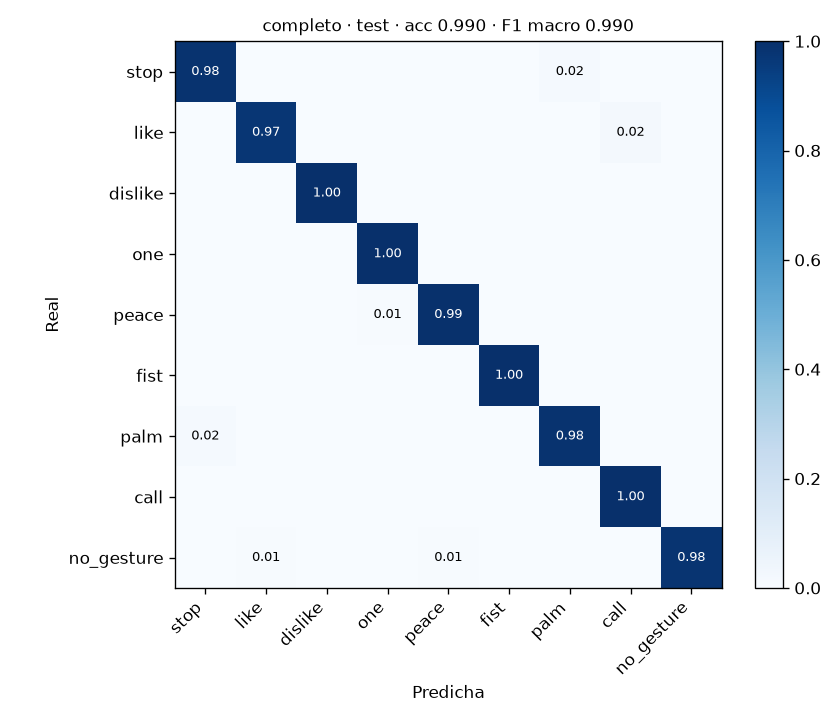
\includegraphics[width=\linewidth]{final/confusion_test.png}
    \captionof{figure}{Matriz de confusión del modelo final en test, normalizada por filas (la
      diagonal es el \emph{recall}).}
    \label{fig:confusion}
  \end{minipage}
\end{figure}

Todas las clases superan el 98\,\% de F1 (\cref{tab:porclase}); la peor es \PeorClaseTest{}
(\PeorFoneTest). Las confusiones más frecuentes (\cref{fig:confusion}) son
\ConfusionesTestFinal. \ErroresEnPares{} de los \ErroresTestFinal{} errores caen en dos pares de
gestos visualmente próximos: \cls{stop}/\cls{palm}, que solo se distinguen por si los dedos están
juntos o separados, y \cls{like}/\cls{call}, que se diferencian por el meñique. Para el robot, el
error más grave es tomar una mano en reposo por una orden: \FalsasActivaciones{} de los
\NNoGestureTest{} ejemplos de \cls{no\_gesture} de test (\TasaFalsasActivaciones) se clasificaron
como algún gesto.

\subsection{Estudio de ablación}
\label{sec:ablacion}

\begin{table}[t]
  \centering
  \caption{Ablación: media de las semillas 42 y 43. Cada variante quita un único componente del
    modelo completo (lotes de 64); la última columna da las épocas de cada semilla.
    $^\dagger$ResNet18 se entrenó una sola vez.}
  \label{tab:ablacion}
  \small
  \setlength{\tabcolsep}{4.5pt}
  \TablaAblacion
\end{table}

La normalización por lotes es la única ablación con un efecto claro (\cref{tab:ablacion}). Sin BN,
la exactitud media en test baja al \AccTestMediaSinBn, frente al \AccTestMediaCompleto, y los
errores se duplican. De las imágenes en las que solo acierta uno de los dos modelos,
\SolocompletoSinBn{} las acierta el completo y \SolovarianteSinBn{} la variante sin BN
(\PmcnemarSinBn). Sin BN el aprendizaje es además mucho más lento: tras la primera época la
exactitud de validación es del \AccepocaunoSinBn, y no supera el 95\,\% hasta la época
\EpocanoventaycincoSinBn{} (la \EpocanoventaycincoCompleto{} en el completo). Con ambas semillas
agotó las 50 épocas sin converger, así que el resultado debe leerse como «con el mismo presupuesto
de épocas».

Quitar el \emph{dropout} (\PmcnemarSinDropout) o el aumento de datos (\PmcnemarSinAug) no tiene
un efecto distinguible de la variación entre ejecuciones: dos ejecuciones idénticas del modelo
completo cometen \ErroresTestCompleto{} y \ErroresTestCompletoS{} errores en test. Su huella está
en la dinámica del entrenamiento. Sin aumento de datos, la red memoriza el conjunto de
entrenamiento, la diferencia entre entrenamiento y validación es la mayor de la ablación
(\BrechaSinAug{} puntos, frente a \BrechaCompleto) y la parada actúa antes (épocas
\EpocasSinAug{} y \EpocasSinAugS).

\subsection{Comparación con ResNet18 y coste}
\label{sec:resnet}

ResNet18 preentrenado alcanza un \AccepocaunoResnet{} de exactitud de validación tras la primera
época (GestureCNN: \AccepocaunoFinal). En test obtiene un \AccTestResnet{} (IC:
\AccTestResnetIC), con \ErroresTestResnet{} errores frente a los \ErroresTestFinal{} de
GestureCNN. La diferencia no es significativa: \SolovarianteResnet{} imágenes las acierta solo
ResNet18 y \SolofinalResnet{} solo GestureCNN (\PmcnemarFinalResnet). El preentrenamiento acelera
la convergencia, pero no podemos afirmar que un modelo con \RatioParams{} veces más parámetros
generalice mejor.

En cuanto al coste, el número de parámetros engaña. GestureCNN tiene \RatioParams{} veces menos
parámetros que ResNet18, pero hace \RatioMacs{} veces más operaciones por imagen (\MacsFinal{}
frente a \MacsResnet{} MACs), porque sus dos primeros bloques trabajan a $128^2$ y $64^2$\,px y
acumulan el \FracMacsPrimerosBloques{} de las operaciones. Aun así, con una sola imagen clasifica
un recorte en \LatCpuFinal{} en la CPU (\CPU) y en \LatCudaFinal{} en la GPU, frente a
\LatCpuResnet{} y \LatCudaResnet{} de ResNet18. Los dos modelos caben holgadamente en los 33\,ms
por fotograma de una cámara a 30\,fps.

\subsection{Explicabilidad con Grad-CAM}
\label{sec:gradcam}

En los aciertos de validación, la activación se concentra sobre la mano, no sobre el fondo ni la
cara, y señala los rasgos de cada gesto: en \cls{call}, por ejemplo, el mapa tiene dos máximos,
sobre el pulgar y sobre el meñique. La \cref{fig:gradcam} muestra los errores más seguros, que son
de tres tipos:
\begin{itemize}
  \item \textbf{Ruido de etiqueta}: un \cls{no\_gesture} que es, de hecho, una palma abierta, y
    que la red clasifica como \cls{palm} con probabilidad 1,00.
  \item \textbf{Objetos con forma de gesto}: un teléfono, o el borde vertical de un mueble junto
    al índice, que la red lee como los dedos de \cls{peace}.
  \item \textbf{Pares próximos o imágenes de baja calidad}: \cls{palm}$\to$\cls{stop} con una
    separación intermedia entre los dedos, \cls{like} de perfil confundidos con \cls{call} o
    \cls{one}, y un \cls{palm} pixelado.
\end{itemize}
En los pares próximos, los mapas de la clase real y de la predicha coinciden: la red mira el lugar
correcto, pero la evidencia es ambigua.

\begin{figure}[t]
  \centering
  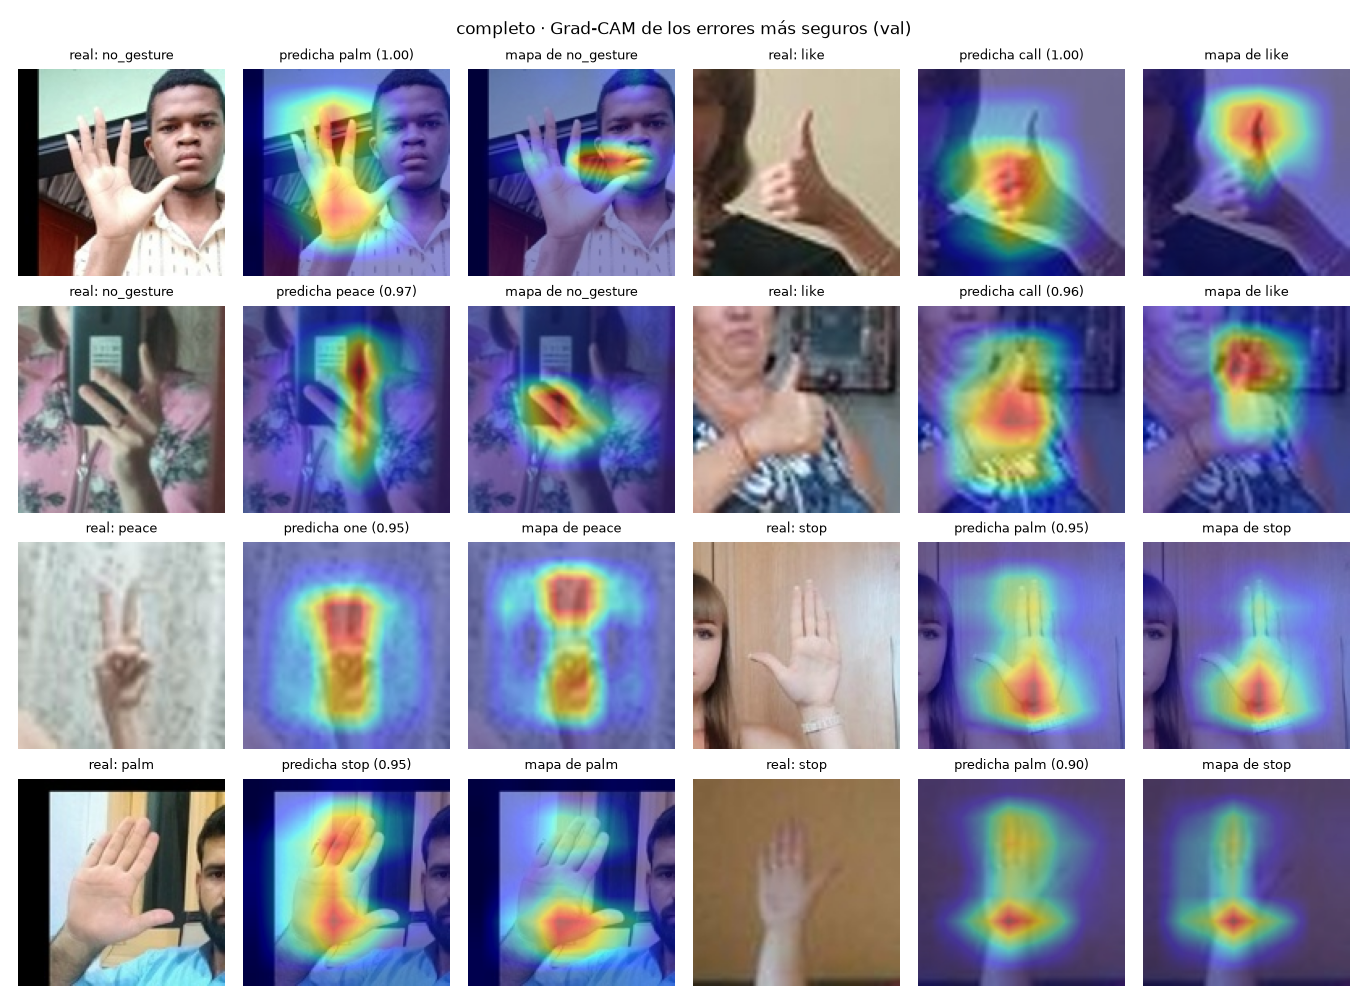
\includegraphics[width=0.85\linewidth]{final/gradcam_errores_val.png}
  \caption{Errores más seguros del modelo final en validación. Para cada uno: la imagen con su
    clase real, el mapa de la clase predicha y el de la clase real.}
  \label{fig:gradcam}
\end{figure}

\section{Demo en tiempo real con un robot simulado}
\label{sec:demo}

Esta sección describe cómo se conecta el clasificador a un robot simulado en ROS\,2
\citep{macenski2022ros2} con \emph{turtlesim}. Usamos \emph{turtlesim} porque recibe las órdenes
de velocidad con la misma interfaz que los robots móviles reales (mensajes \code{Twist} en un
\emph{topic} \code{cmd\_vel}), así que el paso a un simulador como Gazebo, o a un robot físico, no
cambia el nodo de control.

\subsection{Diseño}

El sistema procesa cada fotograma de la cámara en cinco etapas (\cref{fig:pipeline}):
\begin{enumerate}
  \item \textbf{Captura} del fotograma con OpenCV.
  \item \textbf{Detección de la mano} con MediaPipe Hands \citep{zhang2020mediapipe}: la caja se
    obtiene como el rectángulo que envuelve los 21 puntos clave de la mano.
  \item \textbf{Recorte} con la misma función \code{crop\_hand} que se usó para generar los datos
    de entrenamiento (cuadrado, margen del 25\,\%, $128\times128$\,px) y normalización con las
    estadísticas de entrenamiento. Compartir esta función evita una fuente silenciosa de
    discrepancia entre entrenamiento e inferencia.
  \item \textbf{Clasificación} con GestureCNN, que devuelve una probabilidad por clase.
  \item \textbf{Filtrado y control}: una orden solo se emite si la probabilidad máxima supera
    0,7 \emph{y} es la clase mayoritaria en una ventana de los últimos 5--7 fotogramas. Si no se
    cumple, si no se detecta ninguna mano o si la clase es \cls{no\_gesture}, el nodo publica
    velocidad cero. Las velocidades se publican a 10\,Hz en \code{/turtle1/cmd\_vel}.
\end{enumerate}

El filtro de la última etapa responde al segundo requisito de la \cref{sec:introduccion}: un
fotograma aislado mal clasificado, por ejemplo durante la transición entre dos gestos, no debe
mover el robot. El umbral y la ventana intercambian seguridad por tiempo de reacción: a 30
fotogramas por segundo, una ventana de 7 fotogramas añade como mucho unos 0,2\,s de retardo.

\begin{figure}[t]
  \centering
  \begin{tikzpicture}[font=\footnotesize,
      st/.style={draw, rounded corners=2pt, minimum height=1.1cm, text width=1.62cm, align=center, fill=#1},
      arr/.style={-{Stealth[length=2mm]}, thick}]
    \node[st=gray!10]   (cam) {Cámara\\(OpenCV)};
    \node[st=green!12,  right=0.25cm of cam] (mp)  {MediaPipe\\Hands\\{\scriptsize caja de la mano}};
    \node[st=blue!10,   right=0.25cm of mp]  (cr)  {\code{crop\_hand}\\{\scriptsize $128^2$, margen 25\,\%}};
    \node[st=blue!20, text width=1.95cm, right=0.25cm of cr] (cnn) {GestureCNN\\{\scriptsize prob. por clase}};
    \node[st=orange!15, right=0.25cm of cnn] (fil) {Filtro\\{\scriptsize $p>0{,}7$ y voto 5--7}};
    \node[st=red!10,    right=0.25cm of fil] (ros) {Nodo ROS\,2\\{\scriptsize \code{Twist} a 10\,Hz}};
    \foreach \a/\b in {cam/mp,mp/cr,cr/cnn,cnn/fil,fil/ros} \draw[arr] (\a) -- (\b);
  \end{tikzpicture}
  \caption{Etapas de la demo en tiempo real. Las etapas 3 y 4 reutilizan exactamente el
    preprocesado y el modelo evaluados en este trabajo.}
  \label{fig:pipeline}
\end{figure}

\begin{table}[t]
  \centering
  \caption{Correspondencia entre gestos y órdenes para \emph{turtlesim}. Las órdenes de pinza
    no tienen equivalente directo en \emph{turtlesim}.}
  \label{tab:ordenes}
  \small
  \begin{tabular}{lll}
    \toprule
    Gesto & Orden & Acción en \emph{turtlesim} \\
    \midrule
    \cls{like}       & Avanzar               & \code{linear.x} $> 0$ \\
    \cls{dislike}    & Retroceder            & \code{linear.x} $< 0$ \\
    \cls{one}        & Girar a la izquierda  & \code{angular.z} $> 0$ \\
    \cls{peace}      & Girar a la derecha    & \code{angular.z} $< 0$ \\
    \cls{stop}       & Parar                 & velocidad cero \\
    \cls{fist}, \cls{palm} & Cerrar / abrir pinza & sin equivalente (ver texto) \\
    \cls{call}       & Volver al inicio      & servicio \code{teleport\_absolute} \\
    \cls{no\_gesture} & Ninguna              & velocidad cero \\
    \bottomrule
  \end{tabular}
\end{table}

\pendiente{indicar qué acción se asignó finalmente a \cls{fist} y \cls{palm} en \emph{turtlesim}
  (por ejemplo, subir y bajar el lápiz con el servicio \code{set\_pen}) y confirmar los valores
  finales del umbral, de la ventana de voto y de las velocidades lineal y angular.}

\subsection{Implementación y resultados}

\pendiente{describir la implementación del nodo \code{gesture\_controller} (versión de ROS\,2,
  entorno: Ubuntu nativo, máquina virtual o Docker) y cómo se integró el reconocedor con
  MediaPipe.}

\pendiente{tabla de latencias por etapa (captura, MediaPipe, recorte, CNN, filtro y extremo a
  extremo), con la media y el percentil 95 medidos con \code{time.perf\_counter} sobre al menos
  unos cientos de fotogramas, indicando el equipo usado. Como referencia, la etapa de
  clasificación por sí sola tarda \LatCpuFinal{} en CPU y \LatCudaFinal{} en GPU (mediana,
  \cref{tab:coste}).}

\pendiente{resultados cualitativos de la demo: si la tortuga obedece a cada gesto, activaciones
  falsas observadas (sobre todo durante las transiciones entre gestos), efecto del filtro y
  enlace al vídeo de la demostración.}

\section{Discusión}
\label{sec:discusion}

\paragraph{¿Es creíble una exactitud del 99\,\%?}
Una exactitud tan alta debe tratarse con cautela, porque la causa más habitual de resultados
demasiado buenos es una fuga de información entre entrenamiento y test \citep{kaufman2012leakage}.
Nuestro plan de trabajo consideraba de hecho un resultado por encima del 98\,\% como una señal de
alarma. Hemos descartado las fugas más probables:
\begin{enumerate*}[label=(\roman*)]
  \item la partición es por persona y una prueba automática confirma que no hay personas
    compartidas;
  \item las estadísticas de normalización se calculan solo con entrenamiento;
  \item todas las decisiones se tomaron con validación y el test se evaluó una sola vez por
    modelo (con la salvedad, explicada en la \cref{sec:protocolo}, de que el modelo final se
    cambió tras la búsqueda de hiperparámetros, cuando el test ya se había evaluado con el
    anterior); y
  \item validación y test, con personas distintas, dan resultados casi idénticos.
\end{enumerate*}
Creemos que la exactitud alta se explica más bien por la naturaleza de la tarea tal como la
hemos planteado. Los recortes se obtienen de las cajas anotadas a mano, así que la mano siempre
está centrada y completa. Los gestos de HaGRID están posados deliberadamente para la cámara, y
la mayoría de las clases tienen formas claramente distintas. La dificultad residual se concentra en
\cls{stop}/\cls{palm} y \cls{like}/\cls{call} y en las etiquetas ruidosas de \cls{no\_gesture}.

Esta interpretación delimita también el alcance del resultado. La cifra del 99\,\% estima el
rendimiento del \emph{clasificador} sobre recortes de calidad HaGRID con cajas perfectas, no el
del sistema completo con una webcam. En la demo, las cajas vendrán de MediaPipe y estarán peor
centradas, la cámara y la iluminación serán otras y aparecerán posturas de transición entre
gestos que HaGRID no contiene. Es esperable una caída de rendimiento por este cambio de dominio
que nuestro experimento no cuantifica.

\paragraph{Qué aporta cada componente.}
La ablación muestra un resultado menos uniforme de lo que se suele esperar: de los tres
componentes, solo la normalización por lotes tiene un efecto claro sobre la exactitud final. Su
papel es sobre todo de \emph{optimización}: sin BN la red aprende mucho más despacio y no llega a
converger en 50 épocas, en línea con la motivación original de BN como técnica para estabilizar y
acelerar el entrenamiento \citep{ioffe2015bn}. El \emph{dropout} y el aumento de datos son, en
cambio, técnicas de \emph{regularización}, y su efecto se ve en la dinámica del entrenamiento (más
distancia entre entrenamiento y validación y parada más temprana sin ellas) más que en la
exactitud final. Nuestra interpretación es que, en este problema, el modelo completo sobreajusta
poco: tiene muchos ejemplos por clase, clases equilibradas y la parada anticipada ya lo protege.
No es un argumento para eliminar el \emph{dropout} o el aumento de datos. Ambos deberían ganar
importancia ante el cambio de dominio a la webcam (otras cámaras, iluminación y encuadres), que
nuestro conjunto de test no representa; el aumento de datos se diseñó precisamente para simular
esas variaciones.

\paragraph{Sensibilidad a los hiperparámetros.}
La búsqueda muestra que, alrededor de la configuración inicial, el resultado depende poco de los
hiperparámetros: nueve cambios de tasa de aprendizaje, lote, capacidad y activación mueven la
exactitud de validación menos de medio punto, y casi siempre dentro de la variación entre semillas.
El único cambio elegido, el lote de 32, mejoró la validación pero no el test, lo que ilustra el
riesgo de elegir entre muchas configuraciones con un único conjunto de validación pequeño. El
resultado más útil de la búsqueda es otro: con cuatro veces menos parámetros la red rinde igual,
así que la capacidad de GestureCNN no es lo que limita la exactitud.

\paragraph{CNN propia frente a modelo preentrenado.}
La comparación con ResNet18 matiza la idea de que un modelo más grande y preentrenado es siempre
mejor. Con \NTrain{} imágenes de entrenamiento, una tarea bien acotada y entradas de
$128\times128$, una red de \ParamsFinal{} parámetros entrenada desde cero queda a una distancia
que no podemos distinguir del ruido estadístico. El preentrenamiento sí acelera mucho la
convergencia, y podría marcar más diferencia con menos datos o en el cambio de dominio a la
webcam, algo que no hemos medido. Por otra parte, el análisis de coste muestra que el número de
parámetros es una mala medida del coste de inferencia: la red pequeña es la que más operaciones
realiza, porque trabaja a mayor resolución en sus primeras capas.

\paragraph{Limitaciones.}
\begin{itemize}
  \item \textbf{Cajas anotadas.} Todo el entrenamiento y la evaluación usan las cajas de HaGRID.
    No hemos medido el rendimiento con las cajas de un detector ni con vídeo propio, que es el
    escenario real de uso.
  \item \textbf{Resolución.} Al trabajar con la versión de 384\,px, la mayoría de las manos se
    amplían para llegar a $128\times128$ (mediana del lado de la caja: \LadoCajaMediana), lo que
    elimina detalle fino como la posición exacta del meñique, relevante en \cls{like}/\cls{call}.
  \item \textbf{Pocas repeticiones.} Dos semillas por variante bastan para ver la magnitud de la
    variación entre ejecuciones, pero no para estimar con precisión diferencias de pocas décimas.
    La ResNet18 se entrenó una sola vez.
  \item \textbf{Búsqueda de hiperparámetros limitada.} La búsqueda cambia un hiperparámetro cada
    vez, con una sola semilla por configuración, de modo que no explora interacciones y sus
    diferencias son del orden del ruido entre ejecuciones. Además, se hizo solo sobre el modelo
    completo: es posible que otra tasa de aprendizaje mejore alguna variante de la ablación, en
    particular la red sin BN.
  \item \textbf{Ruido de etiqueta en la clase nula.} Algunos \cls{no\_gesture} son en realidad
    gestos (\cref{sec:gradcam}), lo que penaliza al modelo por predicciones correctas y hace que
    la exactitud medida sea una cota algo pesimista en esa clase.
  \item \textbf{Una sola fuente de datos.} Las personas, los fondos y la forma de grabar son los
    de HaGRID; no sabemos cómo se comporta el modelo con otras poblaciones o cámaras.
\end{itemize}

\section{Conclusiones y trabajo futuro}
\label{sec:conclusiones}

Hemos mostrado que una red convolucional pequeña, entrenada desde cero, reconoce un vocabulario
de ocho gestos más una clase nula con una exactitud del \AccTestFinal{} (IC del 95\,\%:
\AccTestFinalIC) en personas que nunca vio durante el entrenamiento. Esto supera con holgura el
objetivo del 85\,\%. Creemos que las claves del resultado son de diseño más que de capacidad:
clasificar
recortes de la mano en lugar del fotograma completo, construir la clase nula con manos de las
mismas imágenes y medir el rendimiento con una partición por persona.

El estudio de ablación, repetido con dos semillas, indica que la normalización por lotes es el
componente imprescindible: sin ella el entrenamiento es mucho más lento y, con el mismo número
de épocas, comete más del doble de errores (\PmcnemarSinBn). El \emph{dropout} y el aumento de
datos modifican la dinámica del entrenamiento como se espera de un regularizador, pero su efecto
sobre la exactitud final es del mismo orden que la variación entre ejecuciones idénticas.

Frente a un ResNet18 preentrenado, con \RatioParams{} veces más parámetros, la diferencia en test
no es estadísticamente significativa (\PmcnemarResnet). Ambos modelos clasifican un recorte
en pocos milisegundos incluso en CPU, de modo que cualquiera de los dos sirve para una aplicación
en tiempo real. Grad-CAM confirma que la red basa sus decisiones en la forma de la mano, y los
errores restantes se deben sobre todo a gestos realmente parecidos, a imágenes de baja calidad y a
ruido de etiqueta.

\paragraph{Trabajo futuro.}
\begin{itemize}
  \item \textbf{Medir el cambio de dominio.} Evaluar el sistema completo con las cajas de
    MediaPipe y con vídeos propios grabados con distintas iluminaciones, y comparar el resultado
    con el de test. Es el experimento que más falta para valorar el uso real.
  \item \textbf{Entrenar con cajas de detector.} Si el cambio de dominio es grande, entrenar con
    recortes generados por MediaPipe, o perturbar más las cajas durante el aumento de datos.
  \item \textbf{Más resolución.} Usar la versión de HaGRID a 512\,px o superior para conservar
    detalle en manos pequeñas, que es lo que distingue \cls{like} de \cls{call}.
  \item \textbf{Clase nula más rica.} Revisar las etiquetas ruidosas de \cls{no\_gesture} y
    añadir posturas de transición entre gestos, que son las que más riesgo tienen de activar una
    orden por error.
  \item \textbf{Robot real.} Pasar de \emph{turtlesim} a Gazebo o a un robot físico, que usa la
    misma interfaz de velocidades.
\end{itemize}

\section*{Reparto del trabajo}
\addcontentsline{toc}{section}{Reparto del trabajo}

El trabajo se repartió por ficheros con contratos fijos entre ambos (\code{src/common.py}), de
modo que cada autor pudiera avanzar con datos o modelos simulados sin esperar al otro.

\begin{itemize}
  \item \textbf{Daniel Rodríguez Alonso}: descarga y verificación de las anotaciones
    (\code{download.py}, \code{show\_boxes.py}), recorte de manos (\code{prepare\_data.py}),
    equilibrado y partición por persona (\code{make\_splits.py}), carga de datos y aumento
    (\code{dataset.py}), evaluación y curvas (\code{evaluate.py}, \code{plot\_curves.py}),
    Grad-CAM (\code{gradcam.py}), análisis estadístico y de coste (\code{analysis.py}) y ejecución
    de los entrenamientos de la ablación y de la referencia.
  \item \textbf{Carlos Falcón Brito}: propuesta inicial del proyecto, arquitectura GestureCNN y
    ResNet18 (\code{model.py}), datos simulados para desarrollar sin el conjunto real
    (\code{mock\_data.py}), bucle de entrenamiento con parada anticipada (\code{train.py}),
    configuraciones de la ablación y lanzador de experimentos (\code{configs/},
    \code{run\_experiments.py}) y demo con ROS\,2 (\cref{sec:demo}).
\end{itemize}

\paragraph{Uso de herramientas de IA.}
Se utilizó un asistente de IA (Claude, de Anthropic) como apoyo en la programación, en la
ejecución de los experimentos y en la redacción de este informe. Todas las cifras proceden de los
ficheros de resultados del repositorio, generados por los \emph{scripts} descritos. La
responsabilidad sobre el contenido corresponde a los autores.

\paragraph{Código.}
El código, las configuraciones, la partición y los resultados están en
\url{https://github.com/danirodriguezz/gestos-cnn-robot}. Las cifras de este documento se generan
automáticamente a partir de \code{results/} con \code{src/analysis.py}.


\bibliographystyle{unsrtnat}
\bibliography{referencias}

\end{document}
